% ==========================================================================
% INFO 4617 Web Data Science -- Week 10: Introduction to APIs: Wikipedia
% (Chapter 10)
% Build:  latexmk -pdf week-10.tex   (from this folder; no env vars needed)
% (or run `make` from the slides/ directory to build every deck)
% ==========================================================================
\documentclass[9pt,aspectratio=169]{beamer}
% Resolve the shared theme/preamble in ../common/ when compiling this
% file directly from its own folder (no TEXINPUTS needed).
\makeatletter\def\input@path{{../common/}}\makeatother
% ==========================================================================
% Shared preamble for INFO 4617 Web Data Science weekly lecture decks
% Based on the Gotham beamer theme (vendored in this directory).
% Each week's slides.tex does:  % ==========================================================================
% Shared preamble for INFO 4617 Web Data Science weekly lecture decks
% Based on the Gotham beamer theme (vendored in this directory).
% Each week's slides.tex does:  % ==========================================================================
% Shared preamble for INFO 4617 Web Data Science weekly lecture decks
% Based on the Gotham beamer theme (vendored in this directory).
% Each week's slides.tex does:  \input{preamble}  (with common/ on TEXINPUTS)
% then sets \title/\subtitle/\author/\date and \begin{document}.
% ==========================================================================

\usetheme{gotham}

\usepackage{fbb}
\usepackage{booktabs}
\usepackage{graphicx}
\usepackage{tikz}
\usepackage{xcolor}
\usepackage{multirow}
\usepackage{listings}
\usetikzlibrary{positioning, arrows.meta, shapes}

% Bibliography
\usepackage[style=authoryear,
            backend=biber,
            maxcitenames=1,
            uniquename=false,
            uniquelist=false]{biblatex}
\addbibresource{bibliography.bib}

\gothamset{sectiontocframe default=off}

% ------------------------------------------------------------------ colors
\definecolor{cugold}{HTML}{CFB87C}
\definecolor{tab-red}{HTML}{E15759}
\definecolor{tab-orange}{HTML}{F28E2B}
\definecolor{tab-blue}{HTML}{4E79A7}
\definecolor{tab-cyan}{HTML}{76B7B2}
\definecolor{tab-green}{HTML}{59A14F}
\definecolor{tab-yellow}{HTML}{EDC948}
\definecolor{tab-purple}{HTML}{B07AA1}
\definecolor{tab-pink}{HTML}{FF9DA7}
\definecolor{tab-brown}{HTML}{9C755F}
\definecolor{tab-gray}{HTML}{BAB0AC}

\setbeamercolor{frametitle}{fg=black, bg=cugold}
\setbeamercolor{progress bar}{fg=cugold, bg=cugold!20}

\setbeamercolor{block title alerted}{fg=black, bg=cugold}
\setbeamercolor{block body alerted}{fg=black, bg=cugold!10}

% ------------------------------------------------------------------ footline
\setbeamertemplate{footline}{
  \begin{beamercolorbox}[wd=\paperwidth,ht=2.5ex,dp=1ex,right]{footline}
    {\footnotesize \insertframenumber{} of \inserttotalframenumber}
    \hspace*{2ex}
  \end{beamercolorbox}
}

% ------------------------------------------------------------------ helpers
\newcommand{\bottomcite}[1]{
    \vspace*{\fill}
    \vspace{-\baselineskip}
    {\tiny
    \rule{\textwidth}{0.3pt}\\
    #1
    }
    \vspace{0.5ex}
}

% Consistent code styling for the Wednesday "applied notebook" frames.
\lstdefinestyle{wds}{
    basicstyle=\ttfamily\scriptsize,
    keywordstyle=\color{tab-blue}\bfseries,
    commentstyle=\color{tab-green},
    stringstyle=\color{tab-orange},
    showstringspaces=false,
    breaklines=true,
    columns=fullflexible,
    language=Python,
    aboveskip=0.4em,
    belowskip=0.4em,
}
\lstset{style=wds}

% \dayband{Day}{Topic} -- a lightweight section divider label used to mark
% Monday / Wednesday / Friday within a week's deck.
\newcommand{\dayband}[2]{{\large\textbf{#1}}\;\textcolor{tab-gray}{\textbar}\;#2}
  (with common/ on TEXINPUTS)
% then sets \title/\subtitle/\author/\date and \begin{document}.
% ==========================================================================

\usetheme{gotham}

\usepackage{fbb}
\usepackage{booktabs}
\usepackage{graphicx}
\usepackage{tikz}
\usepackage{xcolor}
\usepackage{multirow}
\usepackage{listings}
\usetikzlibrary{positioning, arrows.meta, shapes}

% Bibliography
\usepackage[style=authoryear,
            backend=biber,
            maxcitenames=1,
            uniquename=false,
            uniquelist=false]{biblatex}
\addbibresource{bibliography.bib}

\gothamset{sectiontocframe default=off}

% ------------------------------------------------------------------ colors
\definecolor{cugold}{HTML}{CFB87C}
\definecolor{tab-red}{HTML}{E15759}
\definecolor{tab-orange}{HTML}{F28E2B}
\definecolor{tab-blue}{HTML}{4E79A7}
\definecolor{tab-cyan}{HTML}{76B7B2}
\definecolor{tab-green}{HTML}{59A14F}
\definecolor{tab-yellow}{HTML}{EDC948}
\definecolor{tab-purple}{HTML}{B07AA1}
\definecolor{tab-pink}{HTML}{FF9DA7}
\definecolor{tab-brown}{HTML}{9C755F}
\definecolor{tab-gray}{HTML}{BAB0AC}

\setbeamercolor{frametitle}{fg=black, bg=cugold}
\setbeamercolor{progress bar}{fg=cugold, bg=cugold!20}

\setbeamercolor{block title alerted}{fg=black, bg=cugold}
\setbeamercolor{block body alerted}{fg=black, bg=cugold!10}

% ------------------------------------------------------------------ footline
\setbeamertemplate{footline}{
  \begin{beamercolorbox}[wd=\paperwidth,ht=2.5ex,dp=1ex,right]{footline}
    {\footnotesize \insertframenumber{} of \inserttotalframenumber}
    \hspace*{2ex}
  \end{beamercolorbox}
}

% ------------------------------------------------------------------ helpers
\newcommand{\bottomcite}[1]{
    \vspace*{\fill}
    \vspace{-\baselineskip}
    {\tiny
    \rule{\textwidth}{0.3pt}\\
    #1
    }
    \vspace{0.5ex}
}

% Consistent code styling for the Wednesday "applied notebook" frames.
\lstdefinestyle{wds}{
    basicstyle=\ttfamily\scriptsize,
    keywordstyle=\color{tab-blue}\bfseries,
    commentstyle=\color{tab-green},
    stringstyle=\color{tab-orange},
    showstringspaces=false,
    breaklines=true,
    columns=fullflexible,
    language=Python,
    aboveskip=0.4em,
    belowskip=0.4em,
}
\lstset{style=wds}

% \dayband{Day}{Topic} -- a lightweight section divider label used to mark
% Monday / Wednesday / Friday within a week's deck.
\newcommand{\dayband}[2]{{\large\textbf{#1}}\;\textcolor{tab-gray}{\textbar}\;#2}
  (with common/ on TEXINPUTS)
% then sets \title/\subtitle/\author/\date and \begin{document}.
% ==========================================================================

\usetheme{gotham}

\usepackage{fbb}
\usepackage{booktabs}
\usepackage{graphicx}
\usepackage{tikz}
\usepackage{xcolor}
\usepackage{multirow}
\usepackage{listings}
\usetikzlibrary{positioning, arrows.meta, shapes}

% Bibliography
\usepackage[style=authoryear,
            backend=biber,
            maxcitenames=1,
            uniquename=false,
            uniquelist=false]{biblatex}
\addbibresource{bibliography.bib}

\gothamset{sectiontocframe default=off}

% ------------------------------------------------------------------ colors
\definecolor{cugold}{HTML}{CFB87C}
\definecolor{tab-red}{HTML}{E15759}
\definecolor{tab-orange}{HTML}{F28E2B}
\definecolor{tab-blue}{HTML}{4E79A7}
\definecolor{tab-cyan}{HTML}{76B7B2}
\definecolor{tab-green}{HTML}{59A14F}
\definecolor{tab-yellow}{HTML}{EDC948}
\definecolor{tab-purple}{HTML}{B07AA1}
\definecolor{tab-pink}{HTML}{FF9DA7}
\definecolor{tab-brown}{HTML}{9C755F}
\definecolor{tab-gray}{HTML}{BAB0AC}

\setbeamercolor{frametitle}{fg=black, bg=cugold}
\setbeamercolor{progress bar}{fg=cugold, bg=cugold!20}

\setbeamercolor{block title alerted}{fg=black, bg=cugold}
\setbeamercolor{block body alerted}{fg=black, bg=cugold!10}

% ------------------------------------------------------------------ footline
\setbeamertemplate{footline}{
  \begin{beamercolorbox}[wd=\paperwidth,ht=2.5ex,dp=1ex,right]{footline}
    {\footnotesize \insertframenumber{} of \inserttotalframenumber}
    \hspace*{2ex}
  \end{beamercolorbox}
}

% ------------------------------------------------------------------ helpers
\newcommand{\bottomcite}[1]{
    \vspace*{\fill}
    \vspace{-\baselineskip}
    {\tiny
    \rule{\textwidth}{0.3pt}\\
    #1
    }
    \vspace{0.5ex}
}

% Consistent code styling for the Wednesday "applied notebook" frames.
\lstdefinestyle{wds}{
    basicstyle=\ttfamily\scriptsize,
    keywordstyle=\color{tab-blue}\bfseries,
    commentstyle=\color{tab-green},
    stringstyle=\color{tab-orange},
    showstringspaces=false,
    breaklines=true,
    columns=fullflexible,
    language=Python,
    aboveskip=0.4em,
    belowskip=0.4em,
}
\lstset{style=wds}

% \dayband{Day}{Topic} -- a lightweight section divider label used to mark
% Monday / Wednesday / Friday within a week's deck.
\newcommand{\dayband}[2]{{\large\textbf{#1}}\;\textcolor{tab-gray}{\textbar}\;#2}


\title[Week 10 · Wikipedia API]{{\Huge Introduction to APIs: Wikipedia}}
\subtitle{Week 10 · APIs module · Textbook Chapter 10}
\author[Keegan]{\textbf{Brian C. Keegan, Ph.D.} \\ Associate Professor, Department of Information Science \\ University of Colorado Boulder}
\date{October 19, 21 \& 23, 2026}

\begin{document}

\maketitle

% -------------------------------------------------------------------------
\begin{frame}{This week at a glance}
    \begin{columns}[T]
        \begin{column}{0.62\textwidth}
            We leave scraping behind and start asking servers for data \textit{on purpose} --- through a documented API.

            \vspace{0.8em}

            \dayband{Monday}{Concepts \& notebook intro}
            \begin{itemize}\small
                \item What an API is, why it beats scraping, and why we learn on Wikipedia
            \end{itemize}

            \vspace{0.4em}

            \dayband{Wednesday}{Notebook lab}
            \begin{itemize}\small
                \item Query the MediaWiki API: revisions, pageviews, links, raw requests
            \end{itemize}

            \vspace{0.4em}

            \dayband{Friday}{Textbook revisions \textcolor{tab-gray}{\textbar} Proposal due}
            \begin{itemize}\small
                \item Pull requests improving Chapter 10 --- \textbf{and} your Final Project proposal
            \end{itemize}
        \end{column}
        \begin{column}{0.34\textwidth}
            \begin{block}{Companion notebook}
                \footnotesize \texttt{ch-10-wikipedia.ipynb}
            \end{block}
            \begin{alertblock}{Due Friday, Oct 23}
                \footnotesize \textbf{Final Project proposal} --- research question, data source(s), and your API / scraping plan.
            \end{alertblock}
        \end{column}
    \end{columns}
\end{frame}

% =========================================================================
\section{Monday · Concepts}
% =========================================================================

\begin{frame}{From scraping to APIs}
    \begin{columns}[T]
        \begin{column}{0.6\textwidth}
            For six weeks we \textbf{reverse-engineered} pages built for human eyes --- inspecting HTML, guessing selectors, and cleaning up the mess.

            \vspace{1em}

            This week begins Part III: \textbf{API-based data access}. Instead of taking data a site never meant to hand us, we ask for it the way the operator intends.

            \vspace{1em}

            The skills you build here --- reading documentation, constructing parameterized URLs, handling pagination, parsing nested JSON --- transfer to \textit{every} API in the rest of the course.

            \vspace{1em}

            When an API exists, it is almost always the better tool.
        \end{column}
        \begin{column}{0.36\textwidth}
            \centering
            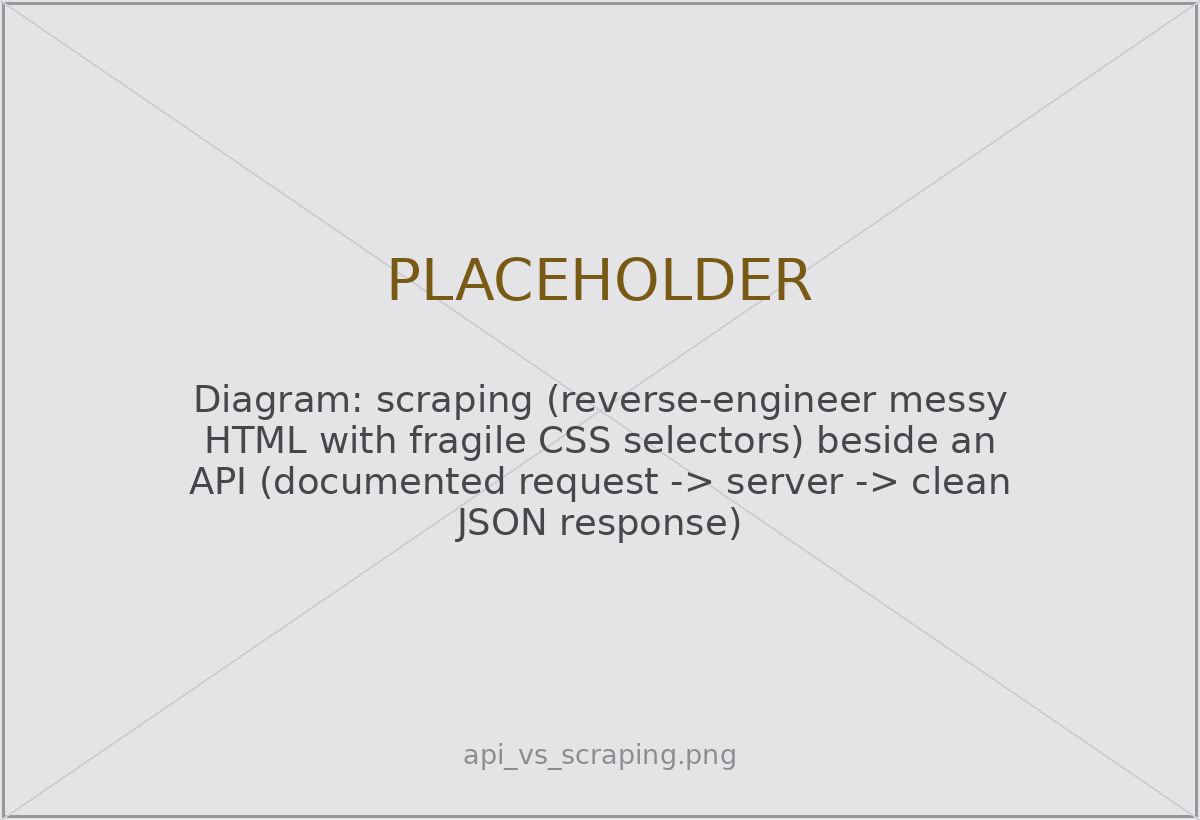
\includegraphics[width=\textwidth]{img/api_vs_scraping.png}\\
            {\scriptsize Ask, don't reverse-engineer.}
        \end{column}
    \end{columns}
    \bottomcite{Textbook Ch.~10, ``From Document Scraping to API Access.''}
\end{frame}

\begin{frame}{What is an API?}
    \begin{columns}[T]
        \begin{column}{0.56\textwidth}
            An \textbf{API} (Application Programming Interface) is a \textbf{contract}: it specifies what you may request, what parameters you may pass, and what format the response will take.

            \vspace{0.8em}

            \begin{itemize}\small
                \item Clean \textbf{JSON}, not cluttered HTML
                \item \textbf{Stable endpoints}, not fragile CSS selectors
                \item \textbf{Documentation} tells you exactly what exists
            \end{itemize}

            \vspace{0.8em}

            The tradeoff: an API only exposes what its operator \textit{chooses} to. You cannot query a missing field, exceed the rate limits, or count on it forever --- the ``post-API age'' (later this module) is a graveyard of APIs that were restricted, repriced, or shut down.
        \end{column}
        \begin{column}{0.4\textwidth}
            \centering
            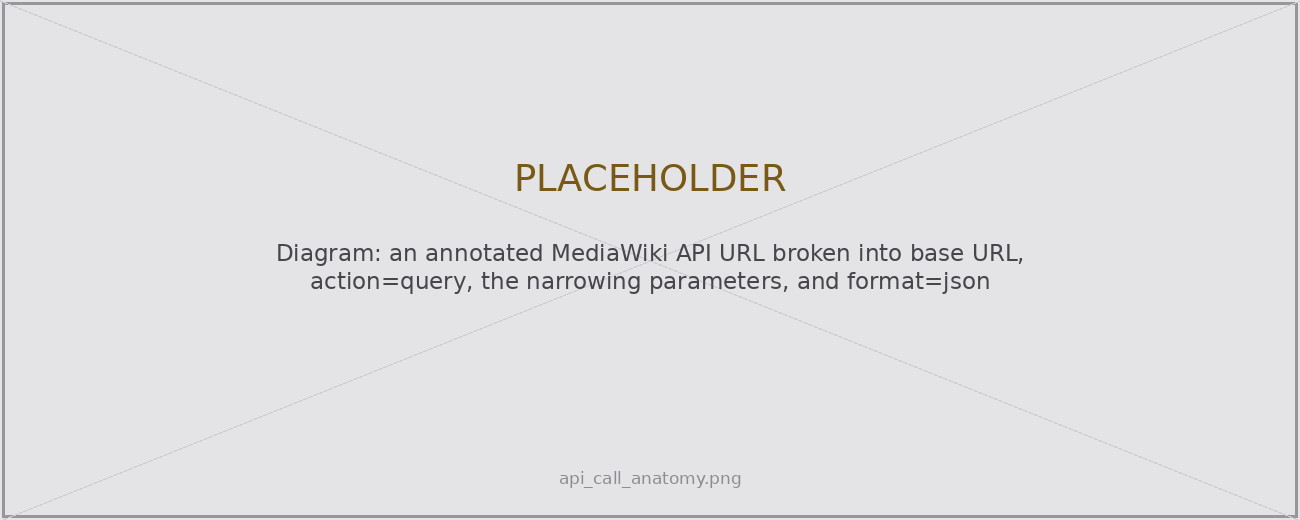
\includegraphics[width=\textwidth]{img/api_call_anatomy.png}\\
            {\scriptsize A request is a URL you assemble on purpose.}
        \end{column}
    \end{columns}
    \bottomcite{Textbook Ch.~10, ``What Is an API?''}
\end{frame}

\begin{frame}{Why Wikipedia?}
    \begin{columns}[T]
        \begin{column}{0.58\textwidth}
            The \textbf{MediaWiki API} is a near-perfect place to learn:
            \begin{itemize}\small
                \item Free, with no authentication beyond a \textbf{User-Agent} header
                \item Comprehensive, well-maintained documentation
                \item Data rich enough for real research --- content, networks, events
            \end{itemize}

            \vspace{0.8em}

            Our case study: the \texttt{Elizabeth\_II} article. Its editing history has dramatic spikes around major events --- ideal for seeing temporal patterns in API data.

            \begin{block}{Public interest}
                \footnotesize Wikipedia is the counter-example to enclosure: an \textbf{open API}, an \textbf{open license}, and public database \textbf{dumps}. Nothing you learn here sits at the mercy of a pricing change.
            \end{block}
        \end{column}
        \begin{column}{0.38\textwidth}
            \centering
            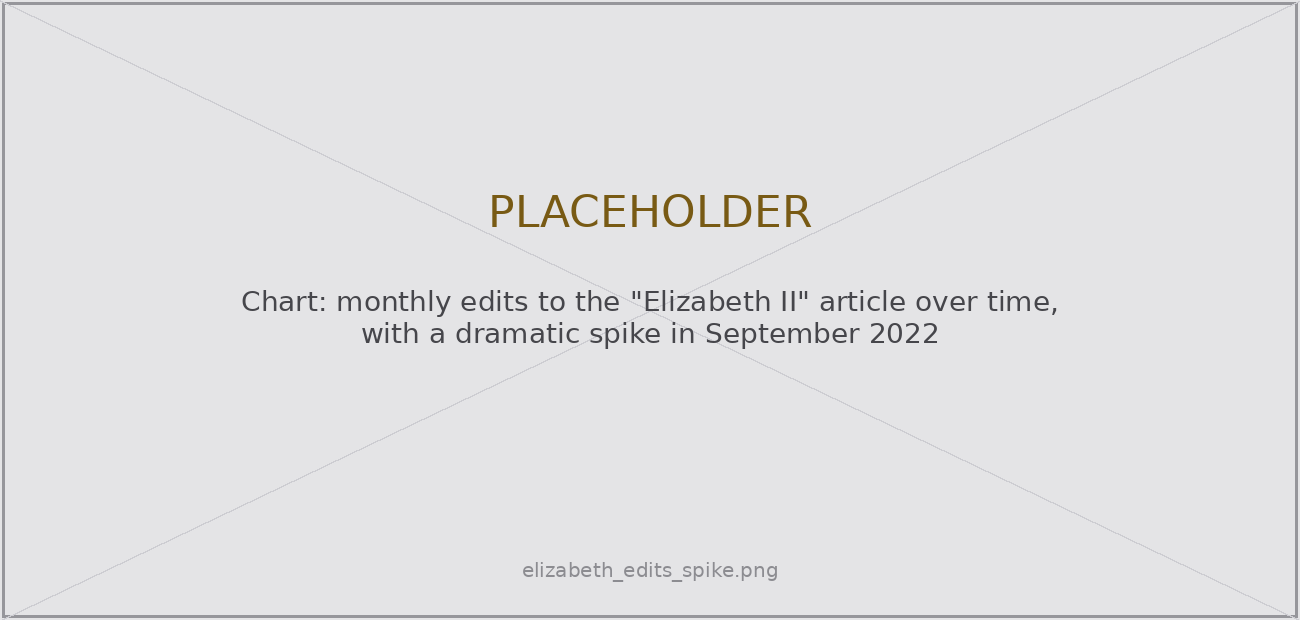
\includegraphics[width=\textwidth]{img/elizabeth_edits_spike.png}\\
            {\scriptsize Every edit, ever, is queryable.}
        \end{column}
    \end{columns}
    \bottomcite{Textbook Ch.~10, ``Why Wikipedia?'' \& the ``Public Interest Connection'' callout.}
\end{frame}

\begin{frame}{The anatomy of a request --- and what the notebook covers}
    \begin{columns}[T]
        \begin{column}{0.54\textwidth}
            Every MediaWiki call is four parts:
            \begin{enumerate}\small
                \item a \textbf{base URL} --- \texttt{.../w/api.php}
                \item an \texttt{\textbf{action}} --- what you want to do
                \item \textbf{parameters} that narrow the request
                \item a \texttt{\textbf{format}} --- \texttt{json}
            \end{enumerate}

            \vspace{0.6em}

            The response is nested JSON you navigate \textbf{one level at a time}: \texttt{data["query"]["pages"][page\_id]}. Internalize that shape once and every endpoint feels familiar.
        \end{column}
        \begin{column}{0.42\textwidth}
            \begin{block}{This week's notebook}
                \footnotesize
                \begin{itemize}\footnotesize
                    \item Revisions + pagination
                    \item Pageviews (a second API)
                    \item Links, categories, languages
                    \item Raw requests from the docs
                \end{itemize}
            \end{block}
            \begin{alertblock}{Connecting to Ch.~2 (Ethics)}
                \footnotesize Identify yourself: the Wikimedia \textbf{User-Agent policy} asks every client for a descriptive agent with contact info. Anonymous traffic gets throttled.
            \end{alertblock}
        \end{column}
    \end{columns}
    \bottomcite{Textbook Ch.~10, ``The Anatomy of an API Call.'' See also \textit{Missing Manual} Ch.~5, ``Reading Official Documentation.''}
\end{frame}

% =========================================================================
\section{Wednesday · Notebook Lab}
% =========================================================================

\begin{frame}[fragile]{The four parts, then navigate the JSON}
    Assemble the request as a dictionary of parameters; \texttt{requests} builds the URL for you:
\begin{lstlisting}
import requests
URL = "https://en.wikipedia.org/w/api.php"
HEADERS = {"User-Agent": "WebDataScience/1.0 (INFO 4617; brian.keegan@colorado.edu)"}

params = {"action": "query",         # what to do
          "titles": "Elizabeth_II",  # about this page
          "prop":   "info",          # what we want back
          "format": "json"}          # how we want it
data = requests.get(URL, params=params, headers=HEADERS).json()
\end{lstlisting}
    Then walk the nested response one key at a time --- page IDs are the keys:
\begin{lstlisting}
pages = data["query"]["pages"]
page_id = list(pages.keys())[0]
print(pages[page_id]["title"], pages[page_id]["pageid"])
\end{lstlisting}
    \bottomcite{Textbook Ch.~10, ``The Anatomy of an API Call.'' Define \texttt{HEADERS} once and reuse it everywhere.}
\end{frame}

\begin{frame}[fragile]{Revisions --- and the pagination loop}
    \begin{columns}[T]
        \begin{column}{0.62\textwidth}
\begin{lstlisting}
def get_revisions(title, headers=HEADERS):
    params = {"action": "query", "titles": title,
        "prop": "revisions", "rvlimit": "max",
        "rvprop": "ids|timestamp|user|size|comment",
        "format": "json"}
    revs = []
    while True:                      # the pagination loop
        data = requests.get(URL, params=params,
                            headers=headers).json()
        page = list(data["query"]["pages"].values())[0]
        revs.extend(page.get("revisions", []))
        if "continue" not in data:   # last batch -> stop
            break
        params.update(data["continue"])  # else: next batch
    return pd.DataFrame(revs)
\end{lstlisting}
        \end{column}
        \begin{column}{0.36\textwidth}
            The single most common API bug: \textbf{forgetting to paginate}. The server returns results in batches (here, capped at 500) and hands back a \texttt{continue} token when more remain.

            \vspace{0.6em}

            Skip the loop and you silently keep a \textit{fraction} of the data.

            \vspace{0.6em}

            Two habits: \texttt{raise\_for\_status()} to fail loudly, and \texttt{maxlag=5} so bulk jobs yield to human readers.
        \end{column}
    \end{columns}
    \bottomcite{Textbook Ch.~10, ``Getting Revisions'' \& ``Understanding Pagination.'' The same loop returns in the government \& social chapters.}
\end{frame}

\begin{frame}[fragile]{Same pattern, more endpoints}
    \begin{columns}[T]
        \begin{column}{0.6\textwidth}
        Pageviews live on a \textbf{different} API (REST) --- parameters are baked into the URL \textit{path}, and there is no continuation:
\begin{lstlisting}
def get_pageviews(title, start, end, headers=HEADERS):
    url = ("https://wikimedia.org/api/rest_v1/metrics"
           "/pageviews/per-article/en.wikipedia"
           f"/all-access/all-agents/{title}"
           f"/daily/{start}/{end}")
    r = requests.get(url, headers=headers)
    r.raise_for_status()
    return pd.DataFrame(r.json()["items"])
\end{lstlisting}
        Links, categories, and languages reuse the \textit{same} Action-API loop --- just swap \texttt{prop} and the matching \texttt{*limit} key (\texttt{links}, \texttt{categories}, \texttt{langlinks}).
        \end{column}
        \begin{column}{0.38\textwidth}
            \centering
            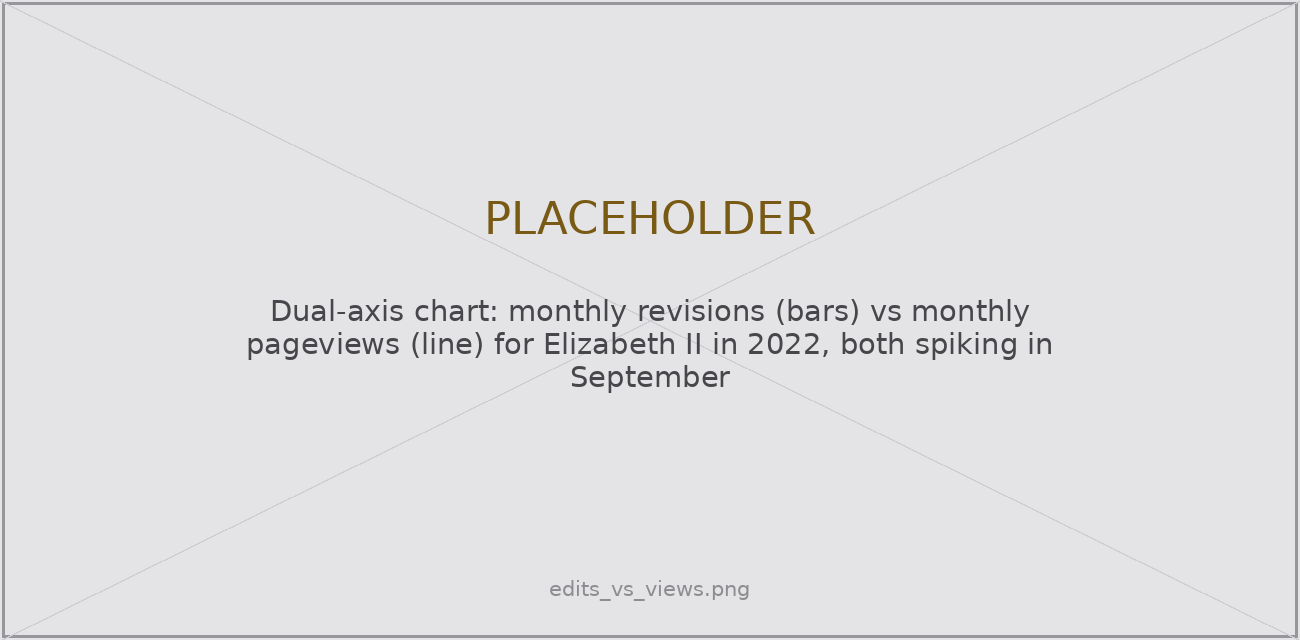
\includegraphics[width=\textwidth]{img/edits_vs_views.png}\\
            {\scriptsize Edits vs.\ views, 2022 --- both spike in September.}

            \vspace{0.5em}
            {\footnotesize How many of Wikipedia's 300+ languages carry an article is a rough proxy for \textbf{global significance} --- one that skews toward the Global North.}
        \end{column}
    \end{columns}
    \bottomcite{Textbook Ch.~10, ``Getting Pageviews,'' ``Getting Links and Categories,'' ``Interlanguage Links.''}
\end{frame}

\begin{frame}[fragile]{From documentation to working code}
    The transferable skill is writing a request from the docs alone --- no wrapper. Read the parameters for an endpoint you have never used, build it, inspect the response:
\begin{lstlisting}
params = {"action": "query",
          "list":   "search",        # a NEW endpoint, learned from the docs
          "srsearch": "web scraping",
          "srlimit": 10,
          "srprop": "wordcount|timestamp|snippet",
          "format": "json"}
data = requests.get(URL, params=params, headers=HEADERS).json()
for r in data["query"]["search"]:
    print(r["title"], "-", r["wordcount"], "words")
\end{lstlisting}
    \begin{columns}[T]
        \begin{column}{0.6\textwidth}
            \footnotesize Libraries like \texttt{mwclient} and \texttt{pywikibot} automate continuation and throttling --- but we write raw requests first so you know exactly what they do for you.
        \end{column}
        \begin{column}{0.36\textwidth}
            \centering
            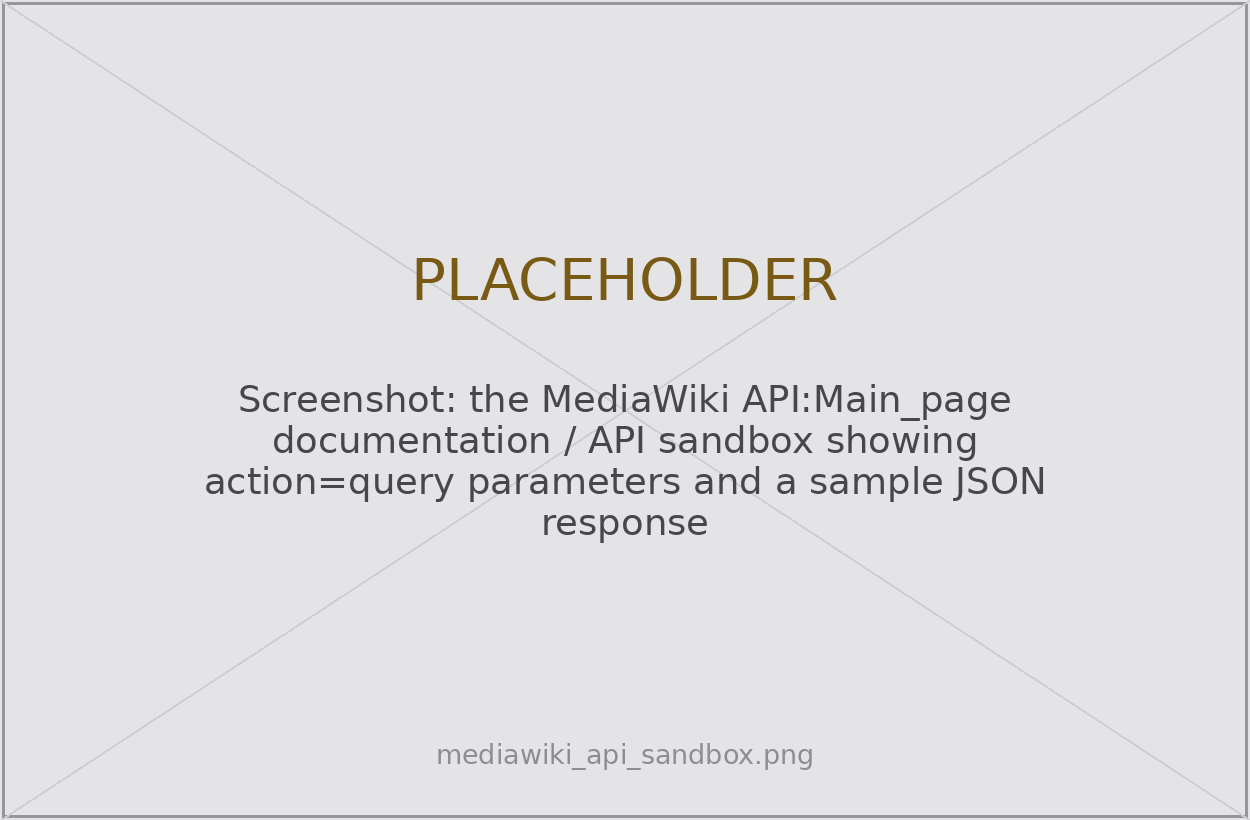
\includegraphics[width=\textwidth]{img/mediawiki_api_sandbox.png}
        \end{column}
    \end{columns}
    \bottomcite{Textbook Ch.~10, ``Writing Raw API Requests from Documentation.''}
\end{frame}

\begin{frame}{Lab: work these, then show-and-tell}
    \begin{columns}[T]
        \begin{column}{0.62\textwidth}
            Work through the chapter's exercises in pairs:
            \begin{enumerate}\small
                \item Compare revision histories of two related articles (unique editors, edits-per-editor, monthly activity)
                \item Detect events: daily pageviews for five articles --- did they spike together or separately?
                \item Link network: overlap of outgoing wikilinks across three related articles
                \item Raw API practice: build a request for a new endpoint (\texttt{extlinks}, \texttt{recentchanges}, \texttt{redirects}) from the docs
                \item Editor network: top-20 editors of an article, then what \textit{else} they edit
                \item[6.] \textcolor{tab-purple}{\textbf{5617}}: reproduce a measure from \textcite{mesgari2015sum} --- e.g.\ a Gini coefficient of edits per editor
            \end{enumerate}
        \end{column}
        \begin{column}{0.34\textwidth}
            \begin{block}{Show-and-Tell}
                \footnotesize Come ready to share:
                \begin{itemize}\footnotesize
                    \item a challenging bug
                    \item interesting data you pulled
                    \item a provocation for a research design
                \end{itemize}
            \end{block}
        \end{column}
    \end{columns}
\end{frame}

\begin{frame}[standout]
    Scraping asks: \textit{how is this page built?}\\
    An API asks: \textit{what does the documentation promise?}\\[1em]
    {\large Learn one API by hand,\\ and you have learned them all.}
\end{frame}

% =========================================================================
\section{Friday · Textbook Revisions}
% =========================================================================

\begin{frame}{Improving Chapter 10 together}
    \begin{columns}[T]
        \begin{column}{0.6\textwidth}
            Today we make the book better. Each of you opens a \textbf{pull request} against \texttt{ch-10-wikipedia.qmd} and reviews a classmate's.

            \vspace{0.6em}

            The workflow (from Week 1):
            \begin{enumerate}\small
                \item Branch / fork the book repo
                \item Edit the chapter; commit with a clear message
                \item Open a PR describing \textit{what} and \textit{why}
                \item Review two peers' PRs: kind, specific, actionable
            \end{enumerate}

            \begin{alertblock}{Also due today --- Fri, Oct 23}
                \footnotesize Submit your \textbf{Final Project proposal}: a research question, your data source(s), and whether you will use an API, scraping, or both.
            \end{alertblock}
        \end{column}
        \begin{column}{0.36\textwidth}
            \centering
            
\includegraphics[width=\textwidth]{img/pr_review.png}
        \end{column}
    \end{columns}
    \bottomcite{Contributions \& reviews count toward the Textbook Revisions grade (30\%).}
\end{frame}

\begin{frame}{A revision menu for Chapter 10}
    High-value targets --- pick one and scope it to a single PR:
    \begin{itemize}
        \item \textbf{Close a gap in ``Common Issues to Debug.''} Add a worked \textbf{missing-page} check (a bad title returns page ID \texttt{-1}), or a \texttt{urllib.parse.quote()} example for titles with parentheses / accents.
        \item \textbf{Show the etiquette, don't just name it.} The chapter mentions \texttt{maxlag} but never demonstrates it --- add a small retry-on-\texttt{maxlag} example for bulk jobs.
        \item \textbf{Add a figure.} A diagram of the request anatomy, or of the request $\rightarrow$ \texttt{continue} $\rightarrow$ request pagination loop, would anchor the two hardest ideas.
        \item \textbf{Strengthen an exercise.} Exercises 1--5 have no expected output or starter cell --- add a rubric or a self-checking assertion.
        \item \textbf{Deepen ``Social History.''} Turn the gender-gap discussion into a reproducible measurement (tie it to WikiProject Women in Red) using this chapter's helper functions.
    \end{itemize}
    \bottomcite{Targets drawn from the chapter's ``Common Issues,'' callouts, thin exercises, and ``Further Reading.''}
\end{frame}

\begin{frame}{What makes a good revision \& a good review}
    \begin{columns}[T]
        \begin{column}{0.48\textwidth}
            \begin{block}{A strong PR}
                \begin{itemize}\small
                    \item One focused change, clearly titled
                    \item Explains the problem it fixes
                    \item Builds (\texttt{quarto render}) without errors
                    \item Matches the book's voice and notation
                    \item Discloses any AI assistance
                \end{itemize}
            \end{block}
        \end{column}
        \begin{column}{0.48\textwidth}
            \begin{block}{A strong review}
                \begin{itemize}\small
                    \item Runs / reads the change, not just skims
                    \item Names specifics (line, claim, code)
                    \item Separates ``must fix'' from ``nice to have''
                    \item Is generous --- assume good faith
                    \item Ends with a clear verdict
                \end{itemize}
            \end{block}
        \end{column}
    \end{columns}
    \vspace{0.5em}
    \centering\small Next week: \textbf{Government APIs} --- the Census, the Federal Reserve (FRED), and other public data services.
\end{frame}

% =========================================================================
\begin{frame}{Key takeaways}
    \begin{enumerate}
        \item An API is a \textbf{documented contract}: structured, intentional access --- clean JSON and stable endpoints, no reverse-engineering.
        \item The skill transfers: \textbf{read the docs $\rightarrow$ build a parameterized request $\rightarrow$ parse nested JSON} one level at a time.
        \item Always \textbf{paginate}: follow the \texttt{continue} token in a loop, or you silently keep only the first batch.
        \item Be a good client: a descriptive \textbf{User-Agent}, serial requests, and \texttt{maxlag} for bulk jobs (the ethics of Ch.~2, applied).
        \item Openness is a \textit{choice}, not a guarantee of completeness --- Wikipedia's data still inherits its volunteer community's biases.
    \end{enumerate}
    \vspace{1em}
    \bottomcite{Reading: Textbook Ch.~10. Further: \textcite{ford2022writing}; \textcite{mesgari2015sum}; \textcite{salganik2018bit}.}
\end{frame}

\end{document}
